\section{Análisis del entorno de depuración del \glsentryshort{bofus}}
\label{sec:ana_gdb}

En esta sección, exploraremos el proceso de depuración del \gls{bofus} utilizando Visual Studio Code (VS Code) y los conocimientos adquiridos sobre el funcionamiento de la interfaz de línea de comandos  del \gls{bofus} en Mininet-WiFi (Ver Sección \ref{sec:ana_bofuss}). El objetivo es comprender en detalle cómo se ejecutan los comandos y qué sucede internamente durante la operación del \gls{bofus} en un entorno de red inalámbrica emulada. En nuestro escenario, trabajaremos con Mininet-WiFi, que nos proporciona un entorno virtualizado para la emulación de redes inalámbricas gracias al modulo del Kernel mac80211\_hwsim. \\
\\
Por ello, trabajaremos en estrecha colaboración con Mininet-WiFi para llevar a cabo la depuración. Sin embargo, este enfoque puede presentar cierta complejidad, por lo que realizaremos una primera aproximación ejecutando el código de una topología sencilla en modo de depuración, lo que nos permitirá observar los comandos que se ejecutan y comprender su funcionamiento. Posteriormente, exploraremos cómo convertir estos comandos en scripts de shell para mayor conveniencia y automatización. Nuestras herramientas de trabajo serán las siguientes:\\

\begin{itemize}
    \item \textbf{Visual Studio Code (VS Code)}: Utilizaremos este editor para escribir y editar el código, así como para realizar la depuración paso a paso. VS Code proporciona una interfaz intuitiva y funciones avanzadas de depuración que nos facilitarán el proceso. A parte de tener una maravillosa terminal integrada y una interfaz con GDB ya desarrollada.

    \item \textbf{Mininet-WiFi}: Esta herramienta nos permitirá emular redes inalámbricas. Trabajaremos con una topología específica, la cual ya hemos mencionado en la sección anterior, y la ejecutaremos en modo de depuración para comprender mejor su funcionamiento, para así poder extraer las lineas de comandos necesarias para replicar su funcionamiento de forma completamente externa.

    \item \textbf{GDB}: Utilizaremos el depurador GDB para analizar y depurar el código del BOFUSS. GDB nos permitirá examinar el estado del programa en tiempo de ejecución, establecer puntos de interrupción, inspeccionar variables y ejecutar el código paso a paso, lo que nos ayudará a identificar posibles errores y problemas en el BOFUSS.
\end{itemize}

Por tanto, vamos a resumir qué estrategia vamos a seguir para depurar al switch. Según se puede apreciar en la Figura \ref{fig:debugBOFUSS}, los pasos que se van a seguir para conseguir depurar al \gls{bofus} son los siguientes. Como se ha indicado, se va a utilizar la misma topología descrita en la Sección \ref{sec:ana_userap}, de las cual se va a obtener la traza de ejecución de la misma. Una vez que se tiene la traza de ejecución de la misma, se desarrrollan dos shell script para levantar el escenario y otro para destruirlo. \\
\\
La idea detrás de esto, es que podamos externalizar el proceso de levantar la topología. Si los scripts son capaces de replicar el funcionamiento de Mininet-WiFi, pasaremos a la siguiente fase, donde se configura el depurador de C que se prefiera, en nuestro caso trabajaremos con GDB. Una vez configurado en VS Code, lanzaremos la el escenario con los scripts previamente programados, y se depurará el funcionamiento del software switch.\\

\newpage

\begin{figure}[ht!]
    \centering
    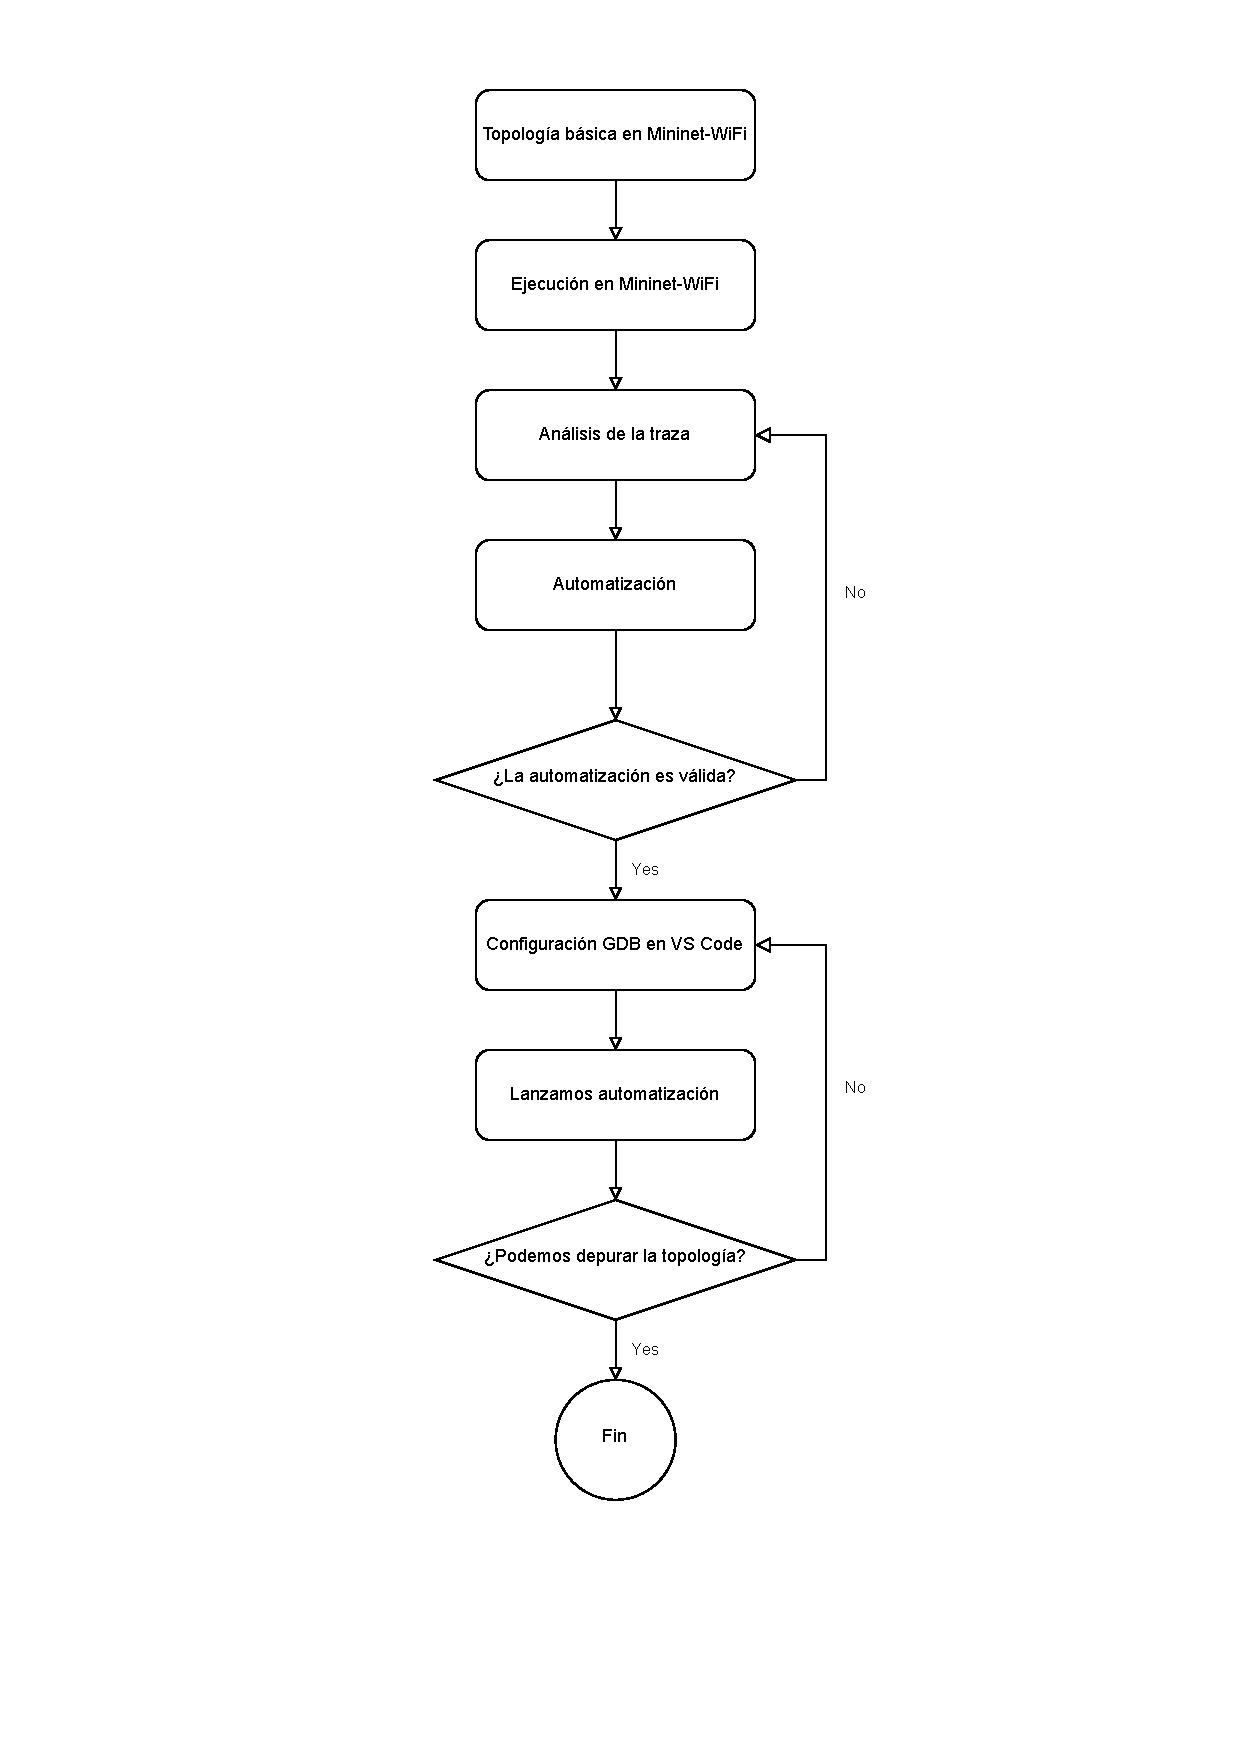
\includegraphics[width=0.9\textwidth]{archivos/img/analisis/debugBOFUSS.drawio.pdf}
    \caption{Proceso de debug al \glsentryshort{bofus}}
    \label{fig:debugBOFUSS}
\end{figure}

\newpage

\subsection{Limpieza del escenario}

La limpieza del escenario es un proceso muy importante dado que la emulación de todos los escenarios que vayamos lanzando se pueden quedar en nuestro equipo haciendo que se consuman recursos o incluso arrojando un comportamiento no esperado haciendo que las conclusiones sobre los desarrollos bajo test sean incorrectos. Para la limpieza del escenario solo hará falta lanzar el siguiente script que únicamente tiene una línea de código (Ver bloque \ref{code:clean}).\\

\begin{lstlisting}[language= bash, style=Consola, caption={Script de limpieza del escenario - clean.sh},label=code:clean]
    # Lanzamos el script de limpieza del propio Mininet
    sudo mn -c
\end{lstlisting}
\vspace{0.5cm}


La simplicidad del script de limpieza es una de sus principales fortalezas. Aunque pueda parecer básico, este script ha sido probado exhaustivamente en una amplia variedad de configuraciones y topologías, demostrando su eficacia para limpiar de forma completa y agnóstica de la topología todos los componentes relacionados con la interfaz wireless.\\
\\
Durante las pruebas realizadas, en una de ellas, se han ejecutado manualmente los comandos para levantar de forma individual la interfaz wireless para el punto de acceso AP1. En este proceso, se ha observado que el script de limpieza elimina correctamente todas las configuraciones previamente establecidas con nuestro shell script. ¿Cuál es el secreto detrás de esta efectividad?\\
\\
Aquí es donde debemos reconocer el trabajo de Ramon Fontes y su contribución en el desarrollo de Mininet-WiFi. Al examinar el contenido\footnote{\href{https://github.com/intrig-unicamp/mininet-wifi/blob/master/mn_wifi/clean.py\#L77}{mininet-wifi/blob/master/mn\_wifi/clean.py-L77}} de la ruta \texttt{/sys/kernel/debug/ieee80211}, se puede encontrar una lista de todas las interfaces inalámbricas emuladas cargadas en el sistema. Es gracias a esta información que el script de limpieza puede identificar y eliminar de manera precisa todas las configuraciones relacionadas con las interfaces wireless, garantizando una limpieza completa. Como se puede ver en la Figura \ref{fig:debugBOFUSS_1}, cuando se lanza el escenario topo.py, al listar las interfaces de la misma forma que lo hace Mininet-WiFi somos capaces de listar todas las interfaces inalámbricas emuladas del sistema, tanto las lanzadas desde Mininet-WiFi como las añadidas a mano haciendo uso de un shell script en paralelo.

\newpage

% fig
\begin{figure}[ht!]
    \centering
    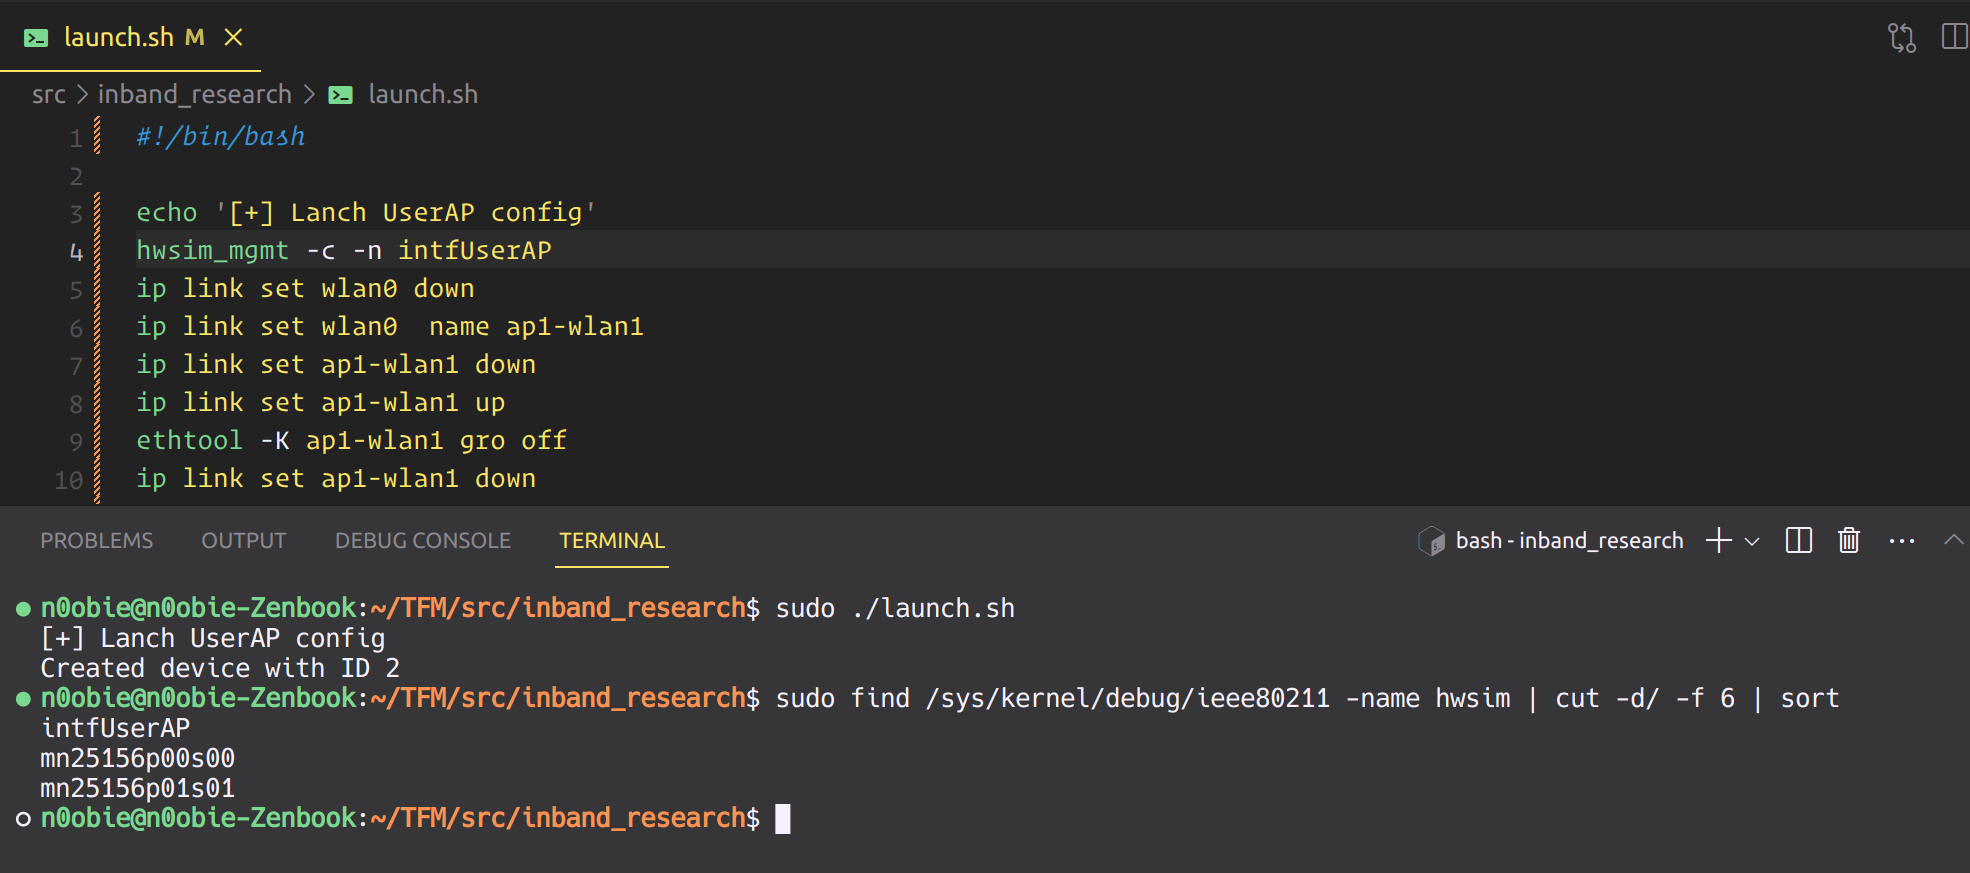
\includegraphics[width=\textwidth]{archivos/img/analisis/debugBOFUSS_1.png}
    \caption{Listado de interfaces inalámbricas en \texttt{/sys/kernel/debug/ieee80211}}
    \label{fig:debugBOFUSS_1}
\end{figure}


Como se puede ver,  como el módulo de limpieza de Mininet-WiFi lee de una ruta desde la cual listan todas las interfaces inalámbricas emuladas, cuando lancemos dicho comando, se listará nuestra capa \textit{phy} emulada, y por ende, será capaz de limpiarla a posteriori.


\subsection{Puesta en marcha del escenario}

Durante el desarrollo del script de puesta en marcha del escenario inalámbrico emulado, se llevó a cabo una exhaustiva investigación para comprender en detalle el funcionamiento interno de la topología básica y la clase \texttt{UserAP} en Mininet-WiFi. Esta investigación fue fundamental para identificar los comandos necesarios y garantizar el correcto funcionamiento del script.\\
\\
Para lograrlo, se analizaron cuidadosamente las trazas de ejecución generadas por el software switch de \texttt{UserAP}. A través de este análisis, se pudo aislar y comprender los comandos utilizados en la creación de radios emuladas. Estas trazas proporcionaron una valiosa información sobre los pasos y procesos involucrados en la configuración de las interfaces inalámbricas. En particular, se observó que la creación de radios emuladas se gestiona mediante la herramienta \texttt{hwsim\_mgmt}. Dentro del código fuente de Mininet-WiFi, este proceso se lleva a cabo en un punto específico y crítico. Este conocimiento fue esencial para extraer los comandos necesarios y adaptarlos al script de lanzamiento del \texttt{UserAP}.\\
\\
El análisis de las trazas y la comprensión del funcionamiento interno de la clase \texttt{UserAP} permitieron obtener una visión clara de los pasos necesarios para configurar y establecer las interfaces inalámbricas emuladas en el escenario. Con esta información en mano, fue posible implementar un script de lanzamiento efectivo que automatiza el proceso y asegura que todas las configuraciones sean aplicadas de manera adecuada (Ver bloque de código \ref{code:launch}).\\

\begin{lstlisting}[language= bash, style=Consola, caption={Script de puesta en marcha del escenario -  launch.sh},label=code:launch]
    #!/bin/bash

    # Vars
    AP_SSID='new-ssid'
    AP_MAC='00:00:00:00:00:01'
    STA_2_CONN=('sta1' 'sta2')

    # Create UserAP
    echo '[+] Lanch UserAP config'
    hwsim_mgmt -c -n intfUserAP
    ip link set wlan0 down
    ip link set wlan0  name ap1-wlan1
    ip link set ap1-wlan1 down 
    ip link set ap1-wlan1 up
    ethtool -K ap1-wlan1 gro off 
    ip link set ap1-wlan1 down 
    ip link set ap1-wlan1 address ${AP_MAC}
    ip link set ap1-wlan1 up
    iw ap1-wlan1 set txpower fixed 100
    echo -e "interface=ap1-wlan1\ndriver=nl80211\nssid=${AP_SSID}\nwds_sta=1\nhw_mode=g\nchannel=1\nctrl_interface=/var/run/hostapd\nctrl_interface_group=0" > mn43736_ap1-wlan1.apconf
    hostapd -B mn43736_ap1-wlan1.apconf
    ip link set ap1-wlan1 down 
    ip link set ap1-wlan1 address ${AP_MAC}
    ip link set ap1-wlan1 up
    tc qdisc replace dev ap1-wlan1 root handle 2: netem rate 54.0000mbit latency 1.00ms
    tc qdisc add dev ap1-wlan1 parent 2:1 handle 10: pfifo limit 1000
    iw dev ap1-wlan1 set txpower fixed 1400
    ofdatapath -i ap1-wlan1 punix:/tmp/ap1 -d 100000000001 --no-slicing 1> /tmp/ap1-ofd.log 2> /tmp/ap1-ofd.log &
    ofprotocol unix:/tmp/ap1 tcp:localhost:6633 --fail=closed  --listen=punix:/tmp/ap1.listen 1> /tmp/ap1-ofp.log 2>/tmp/ap1-ofp.log &

    # Connect stations to AP
    for sta in ${STA_2_CONN[@]}
    do
        echo "[+] Connecting ${sta} to UserAP"
        PID_STA=$(ps aux | grep mininet | grep ${sta} | cut -d' ' -f7)
        echo "[+] ${sta} - Detected pid ${PID_STA}"
        nsenter --target ${PID_STA} --net iwconfig ${sta}-wlan0 essid ${AP_SSID} ap ${AP_MAC}
    done
\end{lstlisting}
\vspace{0.5cm}

Como se puede ver en el bloque de código anterior, primero configuramos lo que viene a ser todos los parámetros propios de la clase \texttt{userAP}, creación de interfaces \textit{wireless} emuladas, configuración de red, además de crear la información requerida con el punto de acceso. Y más adelante lo que se hace es conectar las estaciones WiFi del escenario previamente levantado la red creada por el punto de acceso que se acaba de levantar, accediendo en cada Network namespace de cada estación WiFi.\\
\\
Se quiere añadir un par de detalles que se cree que pueden ser de utilidad al lector en caso de que quieran replicar la depuración \gls{bofus}. Como se ha podido ver para la creación de una radio emulada se tiene que hacer uso del modulo del Kernel mac80211\_hwsim, sin embargo, si se quiere trabajar con el módulo una vez ya insertado en el Kernel tendremos que utilizar otra herramienta. Dicha herrmaienta es \texttt{hwsim\_mgmt}\footnote{\url{https://github.com/patgrosse/mac80211_hwsim_mgmt}}, y a continuación en el bloque de código \ref{code:hwsim} se indican algunos ejemplos de uso de la operativa básica de la herramienta.

\begin{lstlisting}[language= bash, style=Consola, caption={Operativa básica de la herramienta hwsim\_mgmt},label=code:hwsim]
    # Crear una radio emulada
    sudo hwsim_mgmt -c -n [phy_name]

    # Para eliminarlas, se llama a la misma herramienta, de la siguiente manera
    sudo hwsim_mgmt -x [phy_name]
\end{lstlisting}
\vspace{0.5cm}

Es necesario que para trabajar con la herramienta, \texttt{hwsim\_mgmt}, que el modulo del kernel mac80211\_hwsim esté cargado, si no lo está, no podremos crear ninguna radio nueva. En la Figura \ref{fig:debugBOFUSS_2} se ilustra como podemos comprobar si el módulo está previamente cargado. En este caso, si vamos a lanzar primero el script de la topología básica en primera instancia \texttt{topo.py},  el cual ya cargará el modulo, no será necesario tener que cargarlo. Si creamos una interfaz con el modulo ya cargado podemos comprobar que se ha creado un nuevo radio de la siguiente forma (Ver Figura \ref{fig:debugBOFUSS_3}).

% fig
\begin{figure}[ht!]
    \centering
    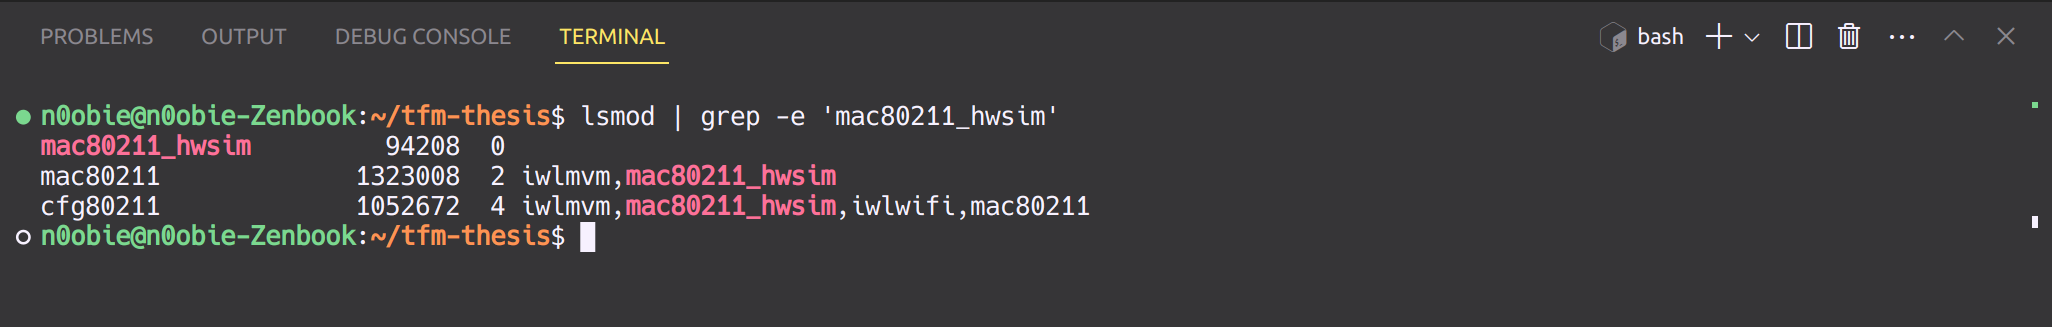
\includegraphics[width=\textwidth]{archivos/img/analisis/debugBOFUSS_2.png}
    \caption{Comprobación de si el módulo \texttt{mac80211\_hwsim} está cargado}
    \label{fig:debugBOFUSS_2}
\end{figure}

% fig
\begin{figure}[ht!]
    \centering
    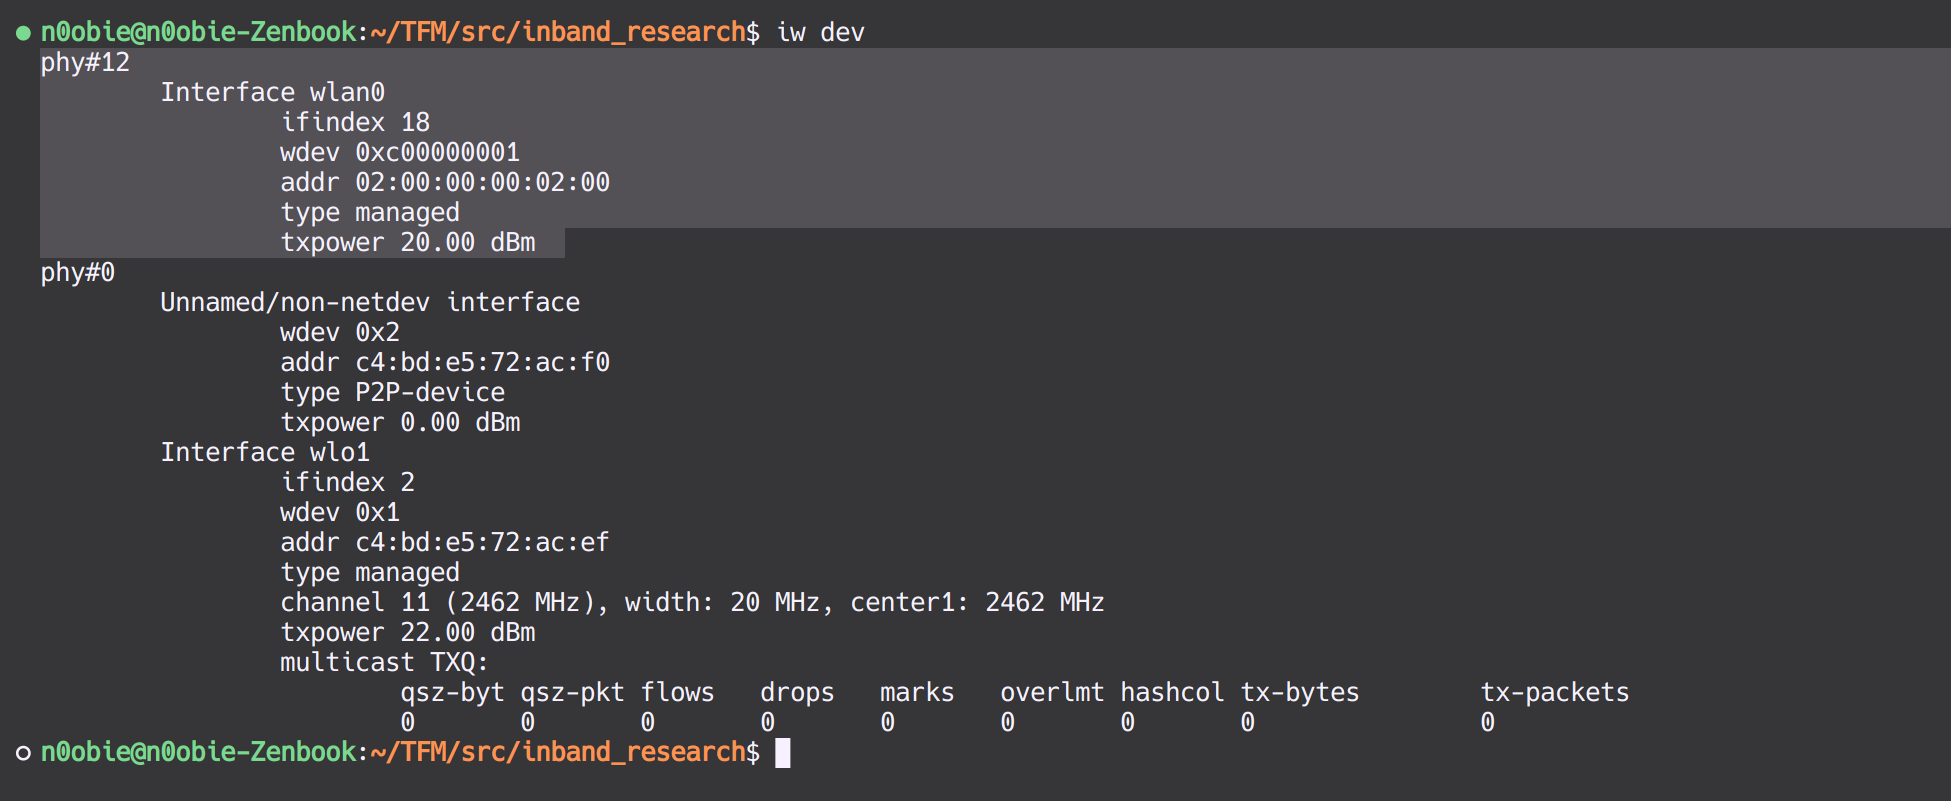
\includegraphics[width=\textwidth]{archivos/img/analisis/debugBOFUSS_3.png}
    \caption{Listado de \textit{phy} inalámbricas usando el comando \texttt{iw}}
    \label{fig:debugBOFUSS_3}
\end{figure}


\subsubsection{Resolución de problemas encontrados}
\label{subsubsec:problemasmalos}
Uno de los problemas más comunes que pueden surgir durante el desarrollo del escenario inalámbrico emulado, es que en algunas ocasiones, nos podemos encontrar con que la interfaz inalámbrica se bloquea y nos muestra un mensaje de advertencia indicando lo siguiente:\\

\begin{lstlisting}[language= bash, style=Consola, caption={Bloqueo de la interfaz por RF-Kill},label=code:rfkills1]
    ~$  Operation not possible due to RF-kill
\end{lstlisting}
\vspace{0.5cm}

Este mensaje indica que la interfaz inalámbrica está bloqueada por una restricción llamada  ``RF-kill". Esta restricción puede ser causada por diferentes factores, como un interrupción mal gestionada, una mala configuración del sistema operativo, o para salvaguardar los recursos de la máquina. Pero generalmente son \textit{soft-blocked} por el Kernel, en la mayoria de los casos para auto-protegerse. Para solucionar este problema, debemos ejecutar el siguiente comando en la terminal (Ver bloque de código \ref{code:rfkills2}).

\begin{lstlisting}[language= bash, style=Consola, caption={desbloqueo de la interfaz por RF-Kill},label=code:rfkills2]
    rfkill unblock all
\end{lstlisting}
\vspace{0.5cm}

Este comando desbloqueará todas las interfaces inalámbricas que estén afectadas por la restricción "RF-kill". Una vez ejecutado el comando, la interfaz inalámbrica estará disponible y podremos establecerla en el estado \texttt{UP} sin problemas.  Si el problema persiste después de ejecutar el comando mencionado, es recomendable verificar otros posibles problemas, como configuraciones incorrectas o conflictos en el sistema.

\subsection{Configuración de VS Code}

Para configurar Visual Studio Code  y poder depurar el \gls{bofus} utilizando GDB, crearemos un archivo JSON con la configuración necesaria. Antes de eso, es importante destacar que hemos logrado lanzar un escenario y ejecutar un UserAP desde un script de shell. Ahora debemos crear un archivo JSON en VS Code que invoque las dos últimas líneas de ofdatapath y ofprotocol para depurar los binarios. Por lo tanto, debemos parametrizar las instrucciones (Líneas del bloque de código \ref{code:bofussLaunch}) en el JSON de depuración. A continuación, en el bloque \ref{code:gdbjson}, se indica el JSON de configuración para la depuración.

\begin{lstlisting}[language= bash, style=Consola, caption={JSON de depuración con GDB del BOFUSS},label=code:gdbjson]
    {
        "version": "0.2.0",
        "configurations": [
            {
                "name": "(ap1)ofprotocol",
                "type": "cppdbg",
                "request": "launch",
                "program": "${workspaceFolder}/secchan/ofprotocol",
                "args": [
                    "unix:/tmp/ap1",
                    "tcp:localhost:6653",
                    "--fail=closed",
                    "--listen=punix:/tmp/ap1.listen"
                ],
                "stopAtEntry": false,
                "cwd": "${workspaceFolder}",
                "environment": [],
                "externalConsole": false,
                "MIMode": "gdb",
                "setupCommands": [
                    {
                        "text": "target-run",
                        "description": "Ofprotocol",
                        "ignoreFailures": true
                    }
                ]
            },
            {
                "name": "(ap1)ofdatapath",
                "type": "cppdbg",
                "request": "launch",
                "program": "${workspaceFolder}/udatapath/ofdatapath",
                "args": [
                    "-i",
                    "ap1-wlan1",
                    "punix:/tmp/ap1",
                    "-d",
                    "000000000001",
                    "--no-slicing"
                ],
                "stopAtEntry": false,
                "cwd": "${workspaceFolder}",
                "environment": [],
                "externalConsole": false,
                "MIMode": "gdb",
                "setupCommands": [
                    {
                        "text": "target-run",
                        "description": "Ofdatapath",
                        "ignoreFailures": true
                    }
                ]
            }
        ],
        "compounds": [
            {
                "name": "(ap1)ofprotocol/(ap1)ofdatapath",
                "configurations": [
                    "(ap1)ofprotocol",
                    "(ap1)ofdatapath"
                ],
                "preLaunchTask": "${defaultBuildTask}",
                "stopAll": true
            }
        ]
    }
\end{lstlisting}
\vspace{0.5cm}


Es importante mencionar que GDB no admite la ejecución con privilegios de root directamente. Para solucionar este problema, es necesario realizar un ajuste adicional\footnote{\url{https://github.com/microsoft/vscode-cmake-tools/issues/2463}}\footnote{\url{https://github.com/microsoft/vscode-cpptools/issues/861}}.